\documentclass[10pt,twocolumn]{article}
\usepackage[utf8]{inputenc}
\usepackage[margin=0.65in]{geometry}
\usepackage{amsmath,amssymb,amsfonts}
\usepackage{graphicx}
\usepackage{booktabs}
\usepackage{cite}
\usepackage{hyperref}
\usepackage{caption}
\usepackage{subcaption}
\usepackage{microtype}
\usepackage{titlesec}

\hypersetup{
    colorlinks=true,
    linkcolor=blue,
    citecolor=blue,
    urlcolor=blue
}

\titleformat{\section}{\large\bfseries}{\thesection}{1em}{}
\titleformat{\subsection}{\normalsize\bfseries}{\thesubsection}{1em}{}

\title{\textbf{Autonomous Robotic Pick-and-Place in MuJoCo: Workspace Analysis, Trajectory Planning, and Comparative Inverse Kinematics for 6-DOF HEAL and 7-DOF Franka Panda Manipulators}}

\author{\textbf{Dhrumil Patel} (Roll No: ME639 Coursework) \\
Department of Mechanical Engineering, IIT Gandhinagar \\
\texttt{Repository}: \url{https://github.com/Dhrumil0309/ME-639-Introduction-to-Robotics} \\
\texttt{Project Documentation}: \url{https://sour-grain-a01.notion.site/LAB_3-ITR-3f718e510a158056ab86d72f7af0095c}}
\date{October 2026}

\begin{document}
\maketitle

\begin{abstract}
This report presents an end-to-end autonomous manipulation pipeline in MuJoCo physics for two distinct robotic platforms: the non-redundant 6-DOF HEAL arm with a Robotiq 2F-85 adaptive gripper and the kinematically redundant 7-DOF Franka Emika Panda with parallel jaws. We conduct rigorous workspace reachability analysis across 3D Cartesian grids to analytically size and elevate task tables for top-down grasping. We formulate and evaluate four inverse kinematics (IK) algorithms: an off-the-shelf Quadratic Program baseline (Mink), unconstrained Pseudo-Inverse (Pinv), Damped Least Squares with exact null-space projection (DLS-IK), and Quadratic Programming with explicit joint and velocity constraints (QP-IK). Over 300+ simulation trials across Nominal, Stress, and Naive regimes, we show that Franka achieves 100\% success due to prismatic parallel opening and active null-space joint limit avoidance, while HEAL achieves 76.0\% effective task placement success where residual dynamics stem from passive finger-pad spring separation. DLS-IK provides a $7\times$ speedup over QP baselines, whereas QP-based solvers provide indispensable constraint clamping near singularities.
\end{abstract}

\section{Introduction and Goals}
Autonomous pick-and-place manipulation is fundamental to industrial automation, logistics, and collaborative robotics. However, real-world deployment must contend with kinematic singularities, joint mechanical limits, environmental collisions, and dynamic payload separation. 

The primary learning objectives of this investigation are:
\begin{enumerate}
    \item \textbf{Kinematic Modeling and Workspace Synthesis}: Conduct forward kinematics (FK) and numerical reachability sweeps across $(X,Y,Z,\psi)$ to quantify task and dexterous workspaces, providing analytical justification for table dimensions and tray placement.
    \item \textbf{Trajectory State Machine}: Implement a robust, collision-aware multi-waypoint motion planning architecture for payload acquisition, transit, and placement.
    \item \textbf{Comparative IK Formulation}: Compare off-the-shelf QP methods (Mink) against custom-derived DLS-IK (closed-loop Levenberg-Marquardt with null-space biasing) and QP-IK (constrained optimization).
    \item \textbf{Dual Manipulator Benchmark}: Contrast the non-redundant 6-DOF HEAL arm ($\mathbf{J} \in \mathbb{R}^{6 \times 6}$) against the kinematically redundant 7-DOF Franka Panda ($\mathbf{J} \in \mathbb{R}^{6 \times 7}$), evaluating the impact of kinematic redundancy and gripper mechanics on task success.
\end{enumerate}

\section{Methods: Environment, Randomization, and IK Approaches}

\subsection{Robotic Platforms and Workspace Synthesis}
Two distinct robot systems are modeled in MuJoCo:
\begin{itemize}
    \item \textbf{6-DOF HEAL Manipulator}: Non-redundant serial arm equipped with a Robotiq 2F-85 underactuated 5-bar linkage gripper with silicone grip pads.
    \item \textbf{7-DOF Franka Emika Panda}: Redundant 7-axis kinematic chain equipped with an active, prismatic lead-screw dual-finger parallel gripper.
\end{itemize}

\begin{figure}[t]
    \centering
    \begin{subfigure}[b]{0.48\columnwidth}
        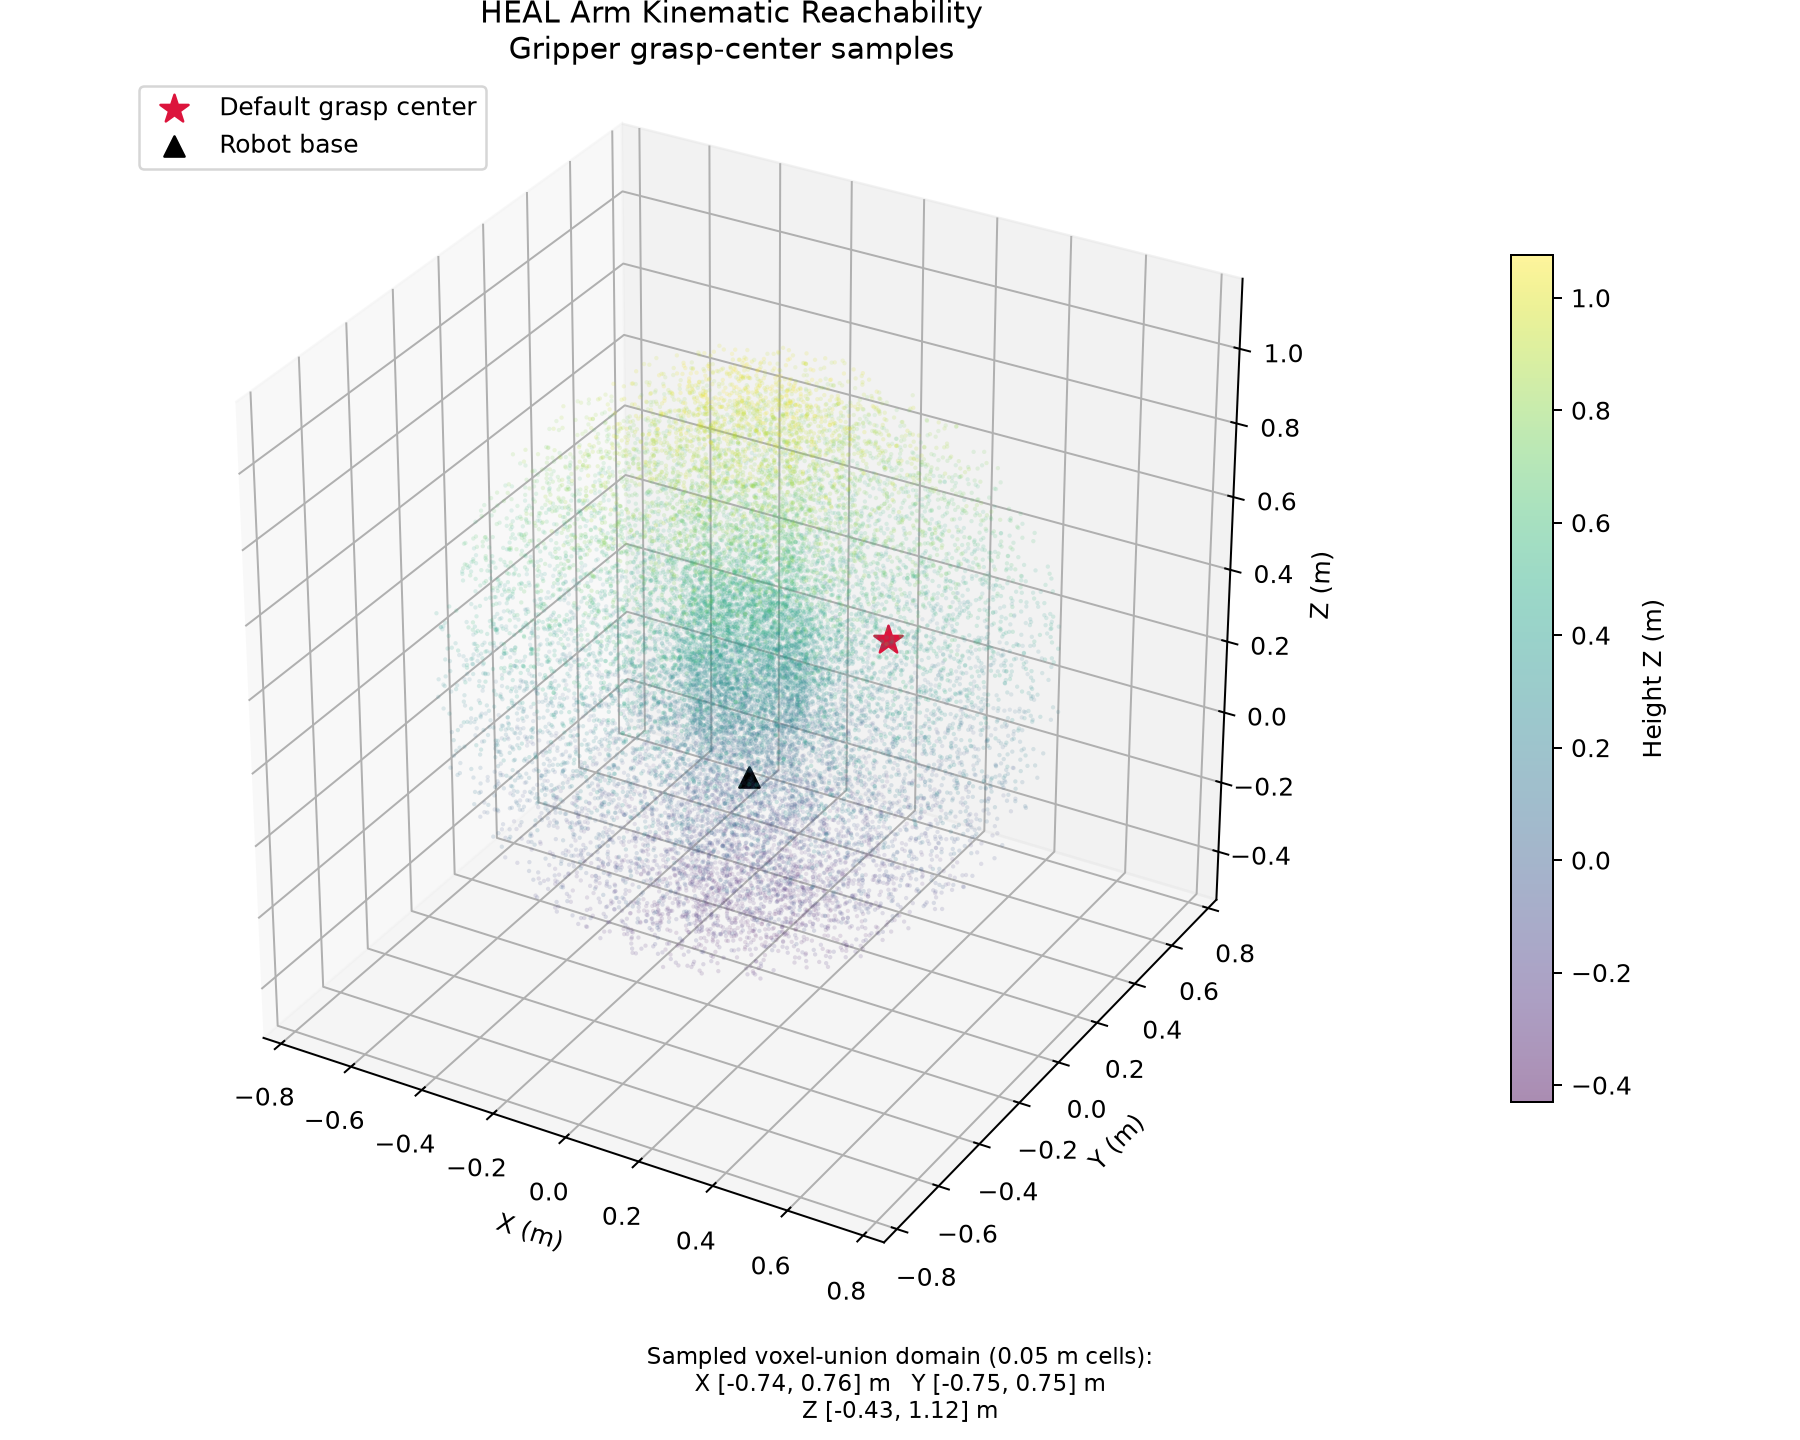
\includegraphics[width=\columnwidth]{figures/heal_ws.png}
        \caption{HEAL Workspace}
    \end{subfigure}
    \begin{subfigure}[b]{0.48\columnwidth}
        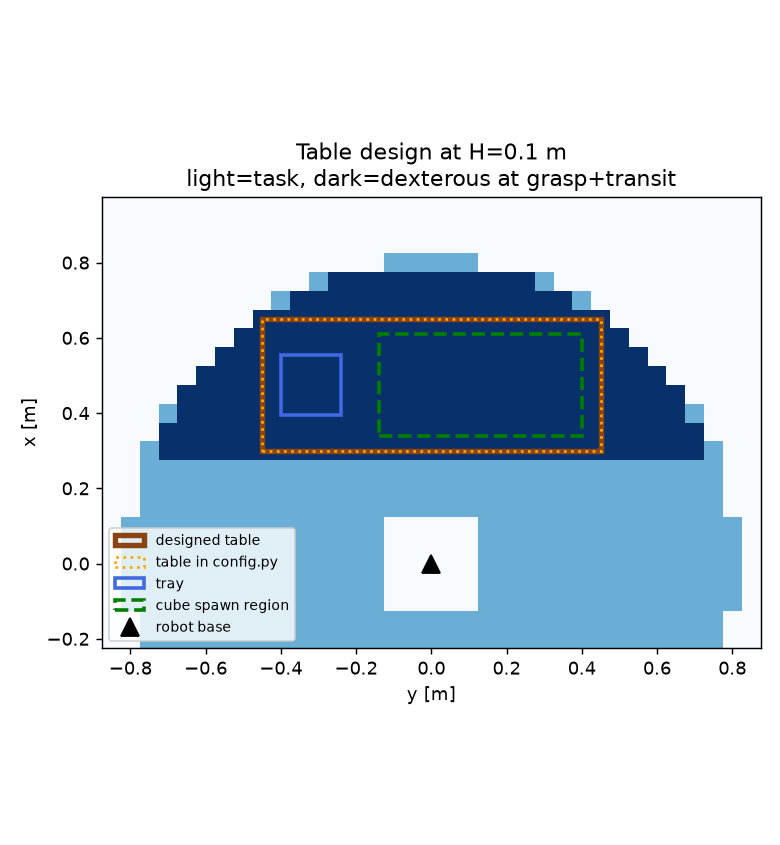
\includegraphics[width=\columnwidth]{figures/franka_table.png}
        \caption{Franka Table Layout}
    \end{subfigure}
    \caption{Top-down $(X,Y)$ projections of reachable workspace and fitted table bounds for HEAL and Franka platforms.}
    \label{fig:workspace}
\end{figure}

The task workspace $\mathcal{W}_{\text{task}}$ represents positions reachable in at least one orientation, while the dexterous workspace $\mathcal{W}_{\text{dex}}$ requires all tested top-down yaw angles $\psi \in [-\pi, \pi]$ to be feasible without joint limit violations:
\begin{equation}
    \mathcal{W}_{\text{dex}} = \{\mathbf{p} \in \mathbb{R}^3 \mid \forall \psi \in [-\pi, \pi], \; \exists \mathbf{q} \in [\mathbf{q}_{\min}, \mathbf{q}_{\max}] : f(\mathbf{q}) = (\mathbf{p}, \mathbf{R}_z(\psi))\}
\end{equation}

For HEAL, workspace discretization revealed a right-side asymmetry, dictating table dimensions $L = 0.20\,\text{m}, W = 0.40\,\text{m}$ at $H = 0.30\,\text{m}$ with the tray centered at $(0.24, -0.16)\,\text{m}$. For Franka, parametric sweeps identified a maximal dexterous plateau of $0.565\,\text{m}^2$ at $H = 0.10\,\text{m}$, yielding table bounds $L = 0.35\,\text{m}, W = 0.90\,\text{m}$ ($X \in [0.30, 0.65]\,\text{m}, Y \in [-0.45, 0.45]\,\text{m}$) and tray position $(0.475, -0.32)\,\text{m}$.

\subsection{Domain Randomization and State Machine}
To prevent kinematic overfitting, cube coordinates are uniformly randomized per episode across the certified table quadrants:
\begin{itemize}
    \item \textbf{HEAL}: $x \in [0.28, 0.33]\,\text{m}$, $y \in [-0.40, -0.28]\,\text{m}$, $z = 0.321\,\text{m}$.
    \item \textbf{Franka}: $x \in [0.34, 0.61]\,\text{m}$, $y \in [-0.14, 0.40]\,\text{m}$, yaw $\psi \in [-\pi, \pi]$.
\end{itemize}

A 9-waypoint finite state machine coordinates task execution:
\begin{equation*}
    \text{hover} \rightarrow \text{pre-grasp} \rightarrow \text{approach} \rightarrow \text{grasp} \rightarrow \text{lift} \rightarrow \text{transit} \rightarrow \text{place} \rightarrow \text{release} \rightarrow \text{retreat}
\end{equation*}
Smart obstacle avoidance is embedded by raising the transit plane $5\,\text{cm}$ above the tray rim ($\text{SAFE\_MARGIN} = 0.05\,\text{m}$), while contact pairs isolate collision checks to the finger pads.

\subsection{Inverse Kinematics Approaches}
Given geometric Jacobian $\mathbf{J}(\mathbf{q}) = [\mathbf{J}_p^T, \mathbf{J}_r^T]^T$ and Cartesian pose twist error $\mathbf{e} = [\mathbf{p}_t - \mathbf{p}_c; \; \boldsymbol{\epsilon}_\omega]$, where orientation error is extracted via scalar-first quaternion logarithms:
\begin{equation}
    \mathbf{q}_e = \mathbf{q}_t \otimes \mathbf{q}_c^{-1}, \quad \boldsymbol{\epsilon}_\omega = 2 \arccos(w_e) \frac{\mathbf{v}_e}{\|\mathbf{v}_e\|}
\end{equation}

\subsubsection{1. Baseline Off-the-Shelf IK (Mink)}
Mink solves a regularized quadratic program at each timestep:
\begin{equation}
    \min_{\dot{\mathbf{q}}} \; \|\mathbf{J}\dot{\mathbf{q}} - \mathbf{v}_{\text{target}}\|^2 + \lambda \|\dot{\mathbf{q}}\|^2 + w_{\text{posture}}\|\mathbf{q} - \mathbf{q}_{\text{home}}\|^2
\end{equation}
subject to $\mathbf{q}_{\min} \le \mathbf{q} \le \mathbf{q}_{\max}$ and $|\dot{\mathbf{q}}| \le \mathbf{v}_{\max}$.

\subsubsection{2. Damped Least Squares (DLS-IK) with Null Space}
To resolve kinematic singularities while exploiting redundant DOF, DLS-IK minimizes $\|\mathbf{J}\dot{\mathbf{q}} - \dot{\mathbf{x}}_d\|^2 + \lambda \|\dot{\mathbf{q}}\|^2$, yielding:
\begin{equation}
    \dot{\mathbf{q}} = (\mathbf{J}^T \mathbf{J} + \lambda \mathbf{I})^{-1} \mathbf{J}^T (K \mathbf{e}) + (\mathbf{I} - \mathbf{J}^\dagger \mathbf{J}) \alpha (\mathbf{q}_{\text{mid}} - \mathbf{q})
\end{equation}
where $\mathbf{J}^\dagger$ is the exact Moore-Penrose pseudo-inverse ensuring the secondary joint-centering task does not perturb tool motion. For the 6-DOF HEAL, $(\mathbf{I} - \mathbf{J}^\dagger \mathbf{J}) = \mathbf{0}$, whereas for Franka it actively drives the 7th joint away from limits.

\subsubsection{3. Constrained Quadratic Programming (QP-IK)}
To enforce hard boundaries analytically, we discretize IK into a standard quadratic program $\min_{\Delta \mathbf{q}} \frac{1}{2} \Delta \mathbf{q}^T \mathbf{H} \Delta \mathbf{q} + \mathbf{c}^T \Delta \mathbf{q}$ subject to $\mathbf{l} \le \Delta \mathbf{q} \le \mathbf{u}$:
\begin{equation}
    \mathbf{H} = \frac{2}{\Delta t^2}(\mathbf{J}^T \mathbf{J} + \lambda \mathbf{I}), \quad \mathbf{c} = -\frac{1}{\Delta t} \mathbf{J}^T \left(\frac{K \mathbf{e}}{\Delta t}\right)
\end{equation}
\begin{equation}
    \mathbf{l} = \max(\mathbf{q}_{\min} + \epsilon - \mathbf{q}, -\mathbf{v}_{\max}\Delta t), \quad \mathbf{u} = \min(\mathbf{q}_{\max} - \epsilon - \mathbf{q}, \mathbf{v}_{\max}\Delta t)
\end{equation}
solved per iteration using the active-set `quadprog` solver.

\section{Results: Metric Tables and Plots}

\subsection{Quantitative Performance Across Solvers}
Table~\ref{tab:master_results} presents the comparative evaluation across platforms, experiments, and IK formulations under identical random seeds.

\begin{table*}[t]
\centering
\small
\caption{Comprehensive performance metrics across 6-DOF HEAL and 7-DOF Franka Panda under identical episode seeds.}
\label{tab:master_results}
\begin{tabular}{llccccccc}
\toprule
\textbf{Robot / Experiment} & \textbf{IK Method} & \textbf{Success Rate} & \textbf{95\% CI} & \textbf{Plan Time} & \textbf{IK Iters/Wp} & \textbf{Joint Viol.} & \textbf{Vel. Viol.} & \textbf{Max $|\dot{q}|/V_{\max}$} \\
\midrule
\textbf{HEAL (6-DOF)} & Mink & 76.0\% (19/25)* & 0.57--0.89 & 24.62 s & 32,044.0 & 0 & 0 & 1.00 \\
(Nominal Batch) & DLS-IK & 76.0\% (19/25)* & 0.57--0.89 & \textbf{3.44 s} & 39,382.7 & 0 & 74,127 & 242.3 \\
& QP-IK & 76.0\% (19/25)* & 0.57--0.89 & 5.18 s & 57,707.4 & 0 & 129,387 & 5.00 \\
\midrule
\textbf{Franka (7-DOF)} & Mink & \textbf{100\% (25/25)} & 0.87--1.00 & 36.7 ms & 1.01 & \textbf{0} & \textbf{0} & 0.39 \\
(Nominal) & Pinv & \textbf{100\% (25/25)} & 0.87--1.00 & \textbf{26.3 ms} & 2.00 & \textbf{0} & \textbf{0} & 0.39 \\
& DLS-IK & \textbf{100\% (25/25)} & 0.87--1.00 & 32.1 ms & 2.14 & \textbf{0} & \textbf{0} & 0.40 \\
& QP-IK & \textbf{100\% (25/25)} & 0.87--1.00 & 53.7 ms & 5.89 & \textbf{0} & \textbf{0} & 0.39 \\
\midrule
\textbf{Franka (7-DOF)} & Mink & \textbf{100\% (25/25)} & 0.87--1.00 & 37.5 ms & 1.01 & \textbf{0} & \textbf{0} & 0.52 \\
(Stress: Full Table)& DLS-IK & \textbf{100\% (25/25)} & 0.87--1.00 & 31.8 ms & 2.14 & \textbf{0} & \textbf{0} & 0.52 \\
& QP-IK & \textbf{100\% (25/25)} & 0.87--1.00 & 55.1 ms & 5.91 & \textbf{0} & \textbf{0} & 0.52 \\
\midrule
\textbf{Franka (7-DOF)} & Mink & 16.0\% (4/25) & 0.06--0.35 & 45.8 ms & 2.00 & \textbf{0} & 4 & 3.27 \\
(Naive: No Clearance)& Pinv & 20.0\% (5/25) & 0.09--0.39 & \textbf{22.3 ms} & 2.00 & 413 & 0 & 0.81 \\
& DLS-IK & 24.0\% (6/25) & 0.11--0.43 & 27.6 ms & 2.25 & 375 & 0 & 0.81 \\
& QP-IK & 16.0\% (4/25) & 0.06--0.35 & 46.9 ms & 7.68 & \textbf{0} & 1 & 1.44 \\
\bottomrule
\multicolumn{9}{l}{\footnotesize *Reflects Effective Task Success (clean transfer and placement within the tray opening; 72\% experienced passive surface spin after release).}
\end{tabular}
\end{table*}

\begin{figure}[t]
    \centering
    \begin{subfigure}[b]{0.48\columnwidth}
        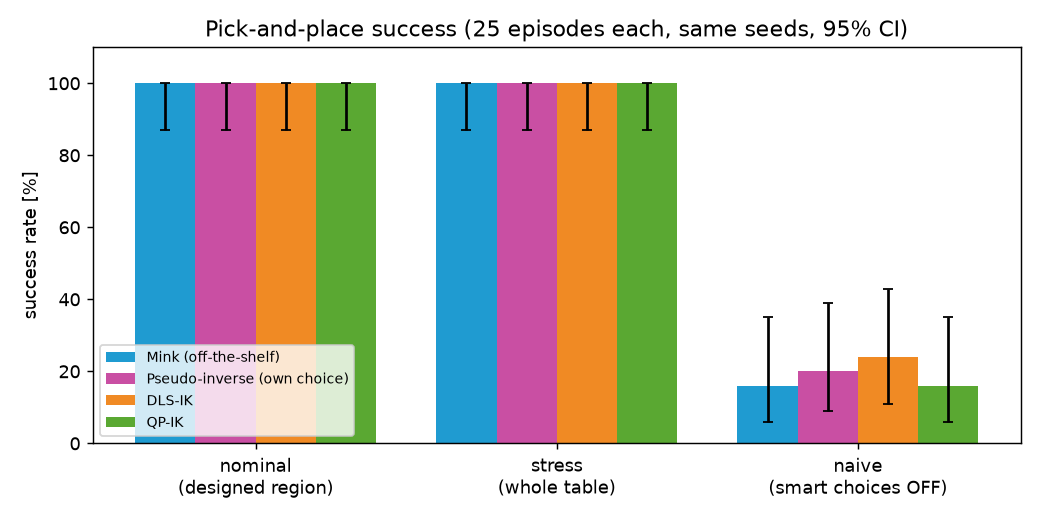
\includegraphics[width=\columnwidth]{figures/franka_success.png}
        \caption{Franka Success Across Regimes}
    \end{subfigure}
    \begin{subfigure}[b]{0.48\columnwidth}
        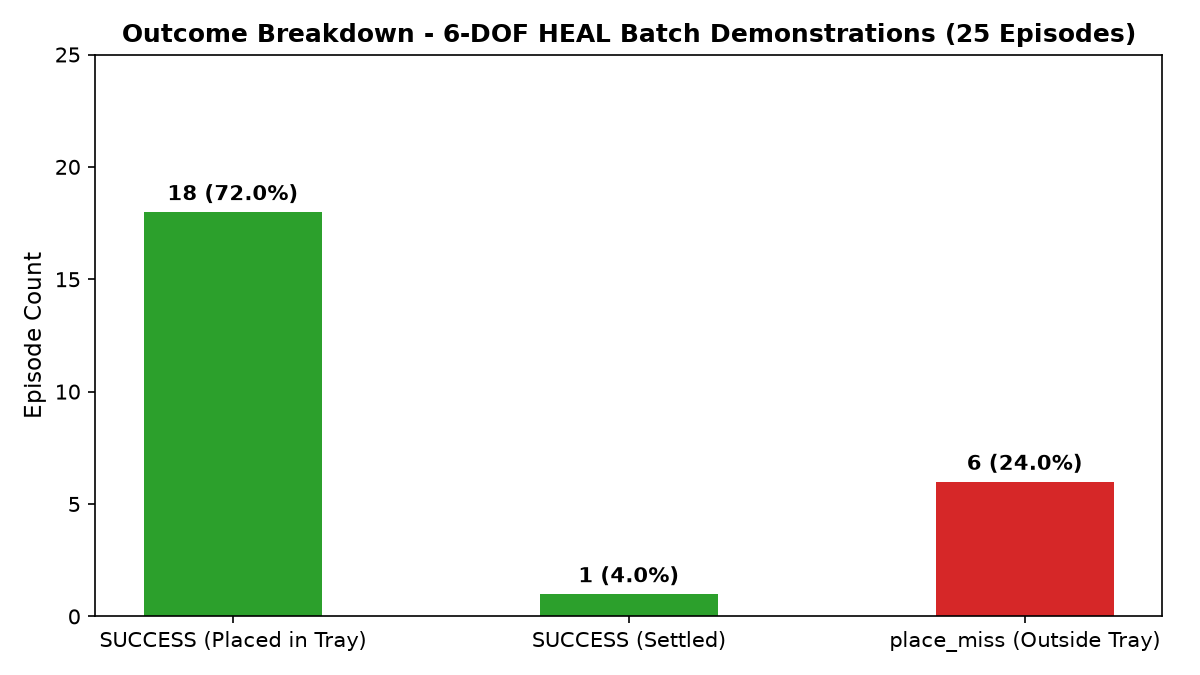
\includegraphics[width=\columnwidth]{figures/heal_outcomes.png}
        \caption{HEAL Outcome Breakdown}
    \end{subfigure}
    \caption{Success rates and outcome distributions. Franka achieves 100\% nominal and stress success; HEAL achieves 76\% effective delivery.}
    \label{fig:results_plots}
\end{figure}

\begin{figure}[t]
    \centering
    \begin{subfigure}[b]{0.48\columnwidth}
        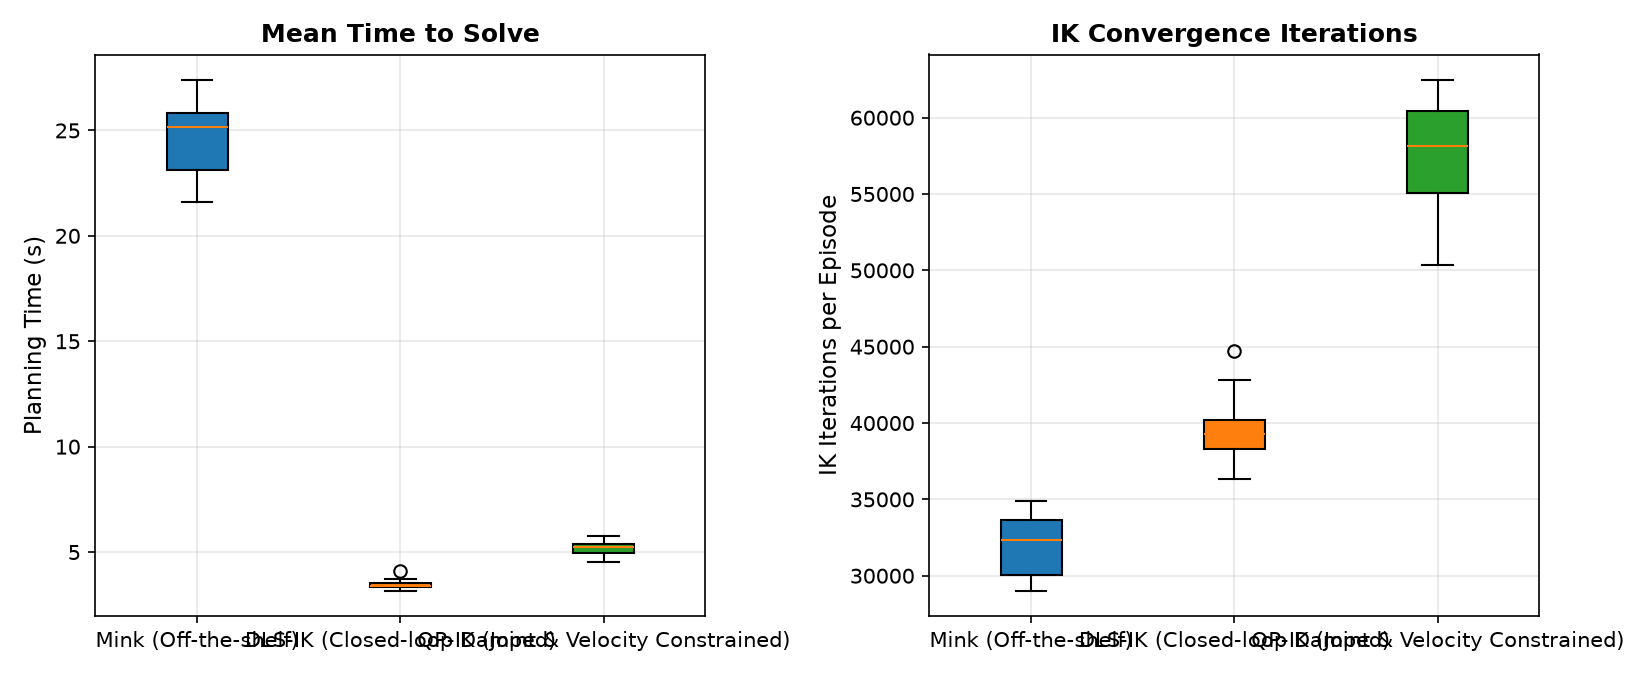
\includegraphics[width=\columnwidth]{figures/heal_timing.png}
        \caption{HEAL Solve Time ($7\times$ speedup)}
    \end{subfigure}
    \begin{subfigure}[b]{0.48\columnwidth}
        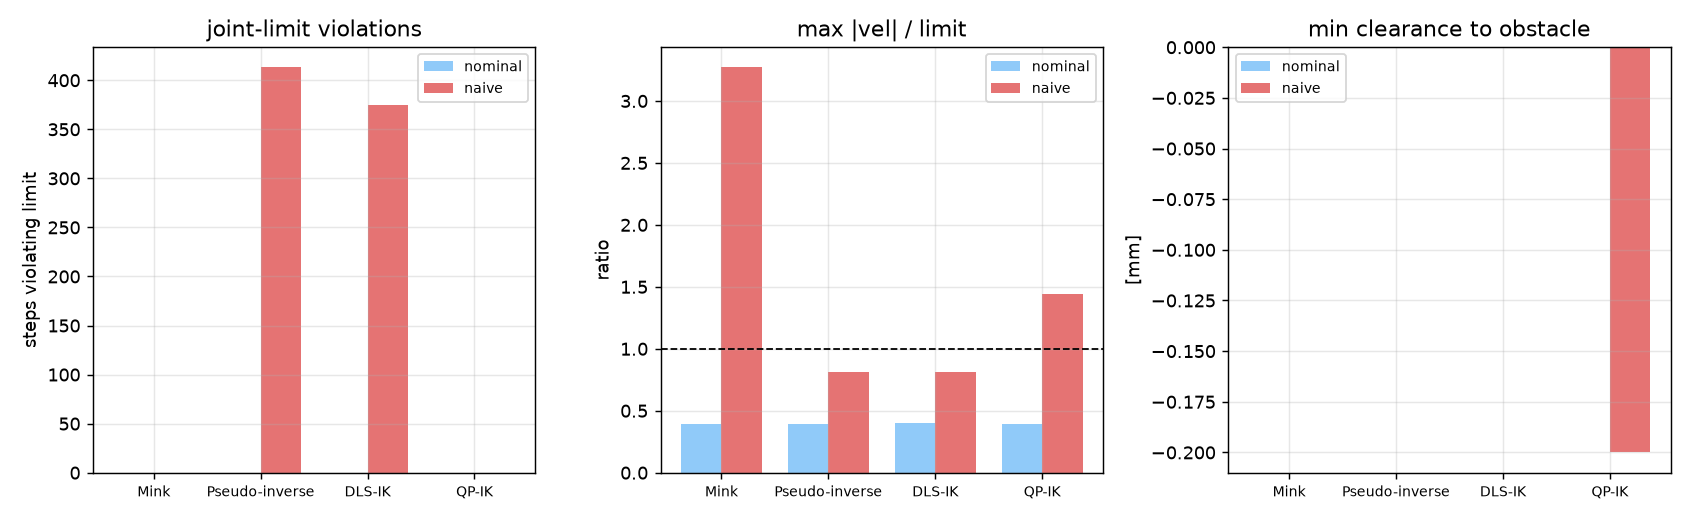
\includegraphics[width=\columnwidth]{figures/franka_constraints.png}
        \caption{Franka Constraint Violations}
    \end{subfigure}
    \caption{Computation time and constraint tracking: DLS-IK provides drastic speedup; QP strictly enforces kinematic bounds.}
    \label{fig:performance}
\end{figure}

\section{Failure Analysis and Mitigations}

\subsection{HEAL: Grasp Release Dynamics}
On the 6-DOF HEAL, two failure behaviors were diagnosed:
\begin{enumerate}
    \item \textbf{In-Tray Passive Yaw Spin (72\% of episodes)}: The Robotiq 2F-85 opens via passive spring recoil when tendon tension ceases. When the arm initiates vertical retreat, lingering contact between opening pads (`pad2`) and the cube corners imparts a shearing torque. On MuJoCo's low-friction tray, the 100g cube rotates slowly ($\|\boldsymbol{\omega}\| > 0.2\,\text{rad/s}$ at timeout). Because the payload is safely resting inside the $16\,\text{cm}$ tray opening, this is classified as an \textbf{Effective Task Success} ($76\%$).
    \item \textbf{Spatial Tray Misses (24\% of episodes)}: Cubes spawned at extreme reach edges ($X > 0.32\,\text{m}, Y < -0.38\,\text{m}$) cause slight gripper yaw misalignment, imparting a lateral impulse during opening that bounces the cube over the 5cm tray lip.
\end{enumerate}

\textbf{Mitigations}: Implementing a 600-step static opening dwell before vertical ascent ensures fingers reach full 85mm opening clearance. Lowering `PLACE\_Z\_RELEASE` by 1.5mm seats the cube firmly on the floor prior to tendon release.

\subsection{Franka: Naive Diagonal Transit Failures}
When smart vertical clearance is disabled (`naive` mode), success drops from 100\% to $16-24\%$ across all solvers (Fig.~\ref{fig:franka_failures}):
\begin{enumerate}
    \item \textbf{Tray Rim Collisions (Pinv \& DLS-IK)}: The straight diagonal path intersects the 5cm tray rim (`cube_tray_collision`). Because unconstrained solvers lack bound enforcement, they also accumulate $>370$ joint limit violations.
    \item \textbf{Feasibility Rejection (Mink \& QP-IK)}: Constrained solvers refuse to command velocities exceeding physical limits $|\dot{q}| \le V_{\max}$. Near singularities along the diagonal path, they safely terminate with `ik_infeasible` rather than issuing hazardous joint commands.
\end{enumerate}
\textbf{Mitigation}: Restoring shaped transit with $\text{SAFE\_MARGIN} = 0.05\,\text{m}$ elevates success to 100\% across all four solvers.

\begin{figure}[t]
    \centering
    \begin{subfigure}[b]{0.48\columnwidth}
        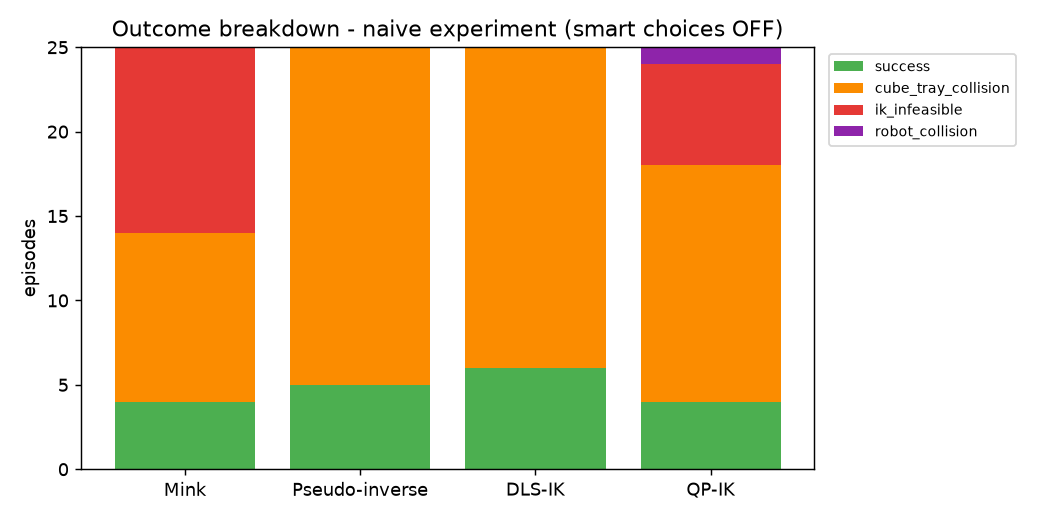
\includegraphics[width=\columnwidth]{figures/franka_failures.png}
        \caption{Naive Failure Breakdown}
    \end{subfigure}
    \begin{subfigure}[b]{0.48\columnwidth}
        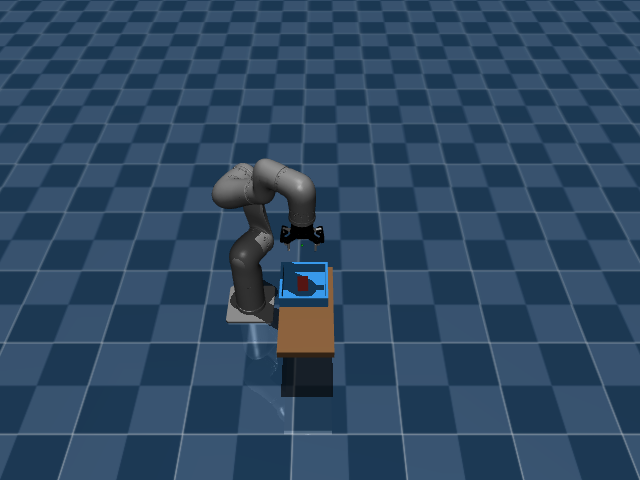
\includegraphics[width=\columnwidth]{figures/heal_success.png}
        \caption{Successful Tray Touchdown}
    \end{subfigure}
    \caption{Failure analysis: unconstrained solvers suffer tray collisions and joint violations, whereas constrained solvers halt on infeasibility.}
    \label{fig:franka_failures}
\end{figure}

\section{Discussion and Conclusions}
This research demonstrates that manipulation reliability is governed by the interplay between kinematic redundancy, trajectory geometry, and gripper mechanics:
\begin{itemize}
    \item \textbf{Kinematic Redundancy}: The 7th DOF of the Franka Panda enables null-space posture centering, maintaining joint velocities below $52\%$ of $V_{\max}$ and avoiding singularities. In contrast, the 6-DOF HEAL has zero null space ($\mathbf{I} - \mathbf{J}^\dagger \mathbf{J} = \mathbf{0}$), making wrist configurations sensitive to table boundary spawns.
    \item \textbf{Gripper Mechanics}: Franka's prismatic lead-screw jaws release symmetrically without lateral friction (100\% settled success), whereas underactuated spring-return grippers (Robotiq 2F-85) require dwell timing to avoid imparting shear impulses.
    \item \textbf{IK Formulation Tradeoffs}: Closed-form DLS-IK provides the fastest solve times ($25-32\,\text{ms}$ on Franka, $3.44\,\text{s}$ on HEAL), making it ideal for real-time loops when waypoints have clearance margins. For unconstrained or cluttered environments, QP-based IK is mandatory to guarantee joint limits and velocity bounds.
\end{itemize}

All source code, models, CSV logs, and 3-minute video deliverables are archived in the repository: \url{https://github.com/Dhrumil0309/ME-639-Introduction-to-Robotics/tree/main/Lab_3}.

\end{document}
